% ============================================================================
% Section 3 - System Architecture
% Packages used: graphicx, booktabs, tabularx
% Upload figures/architecture.pdf to the Overleaf project (folder "figures").
% ============================================================================
\section{System Architecture}
\label{sec:architecture}

Figure~\ref{fig:architecture} shows the complete system. The centre column is the
inference path, which runs for the test word of every fold. The right column is
the training path, which never sees the test word. Colours mark what is learned:
\textbf{orange} components have parameters updated by training, \textbf{grey}
components are frozen or have no parameters, and \textbf{dashed blue} components
are settings chosen without the test word.

\begin{figure}[t]
  \centering
  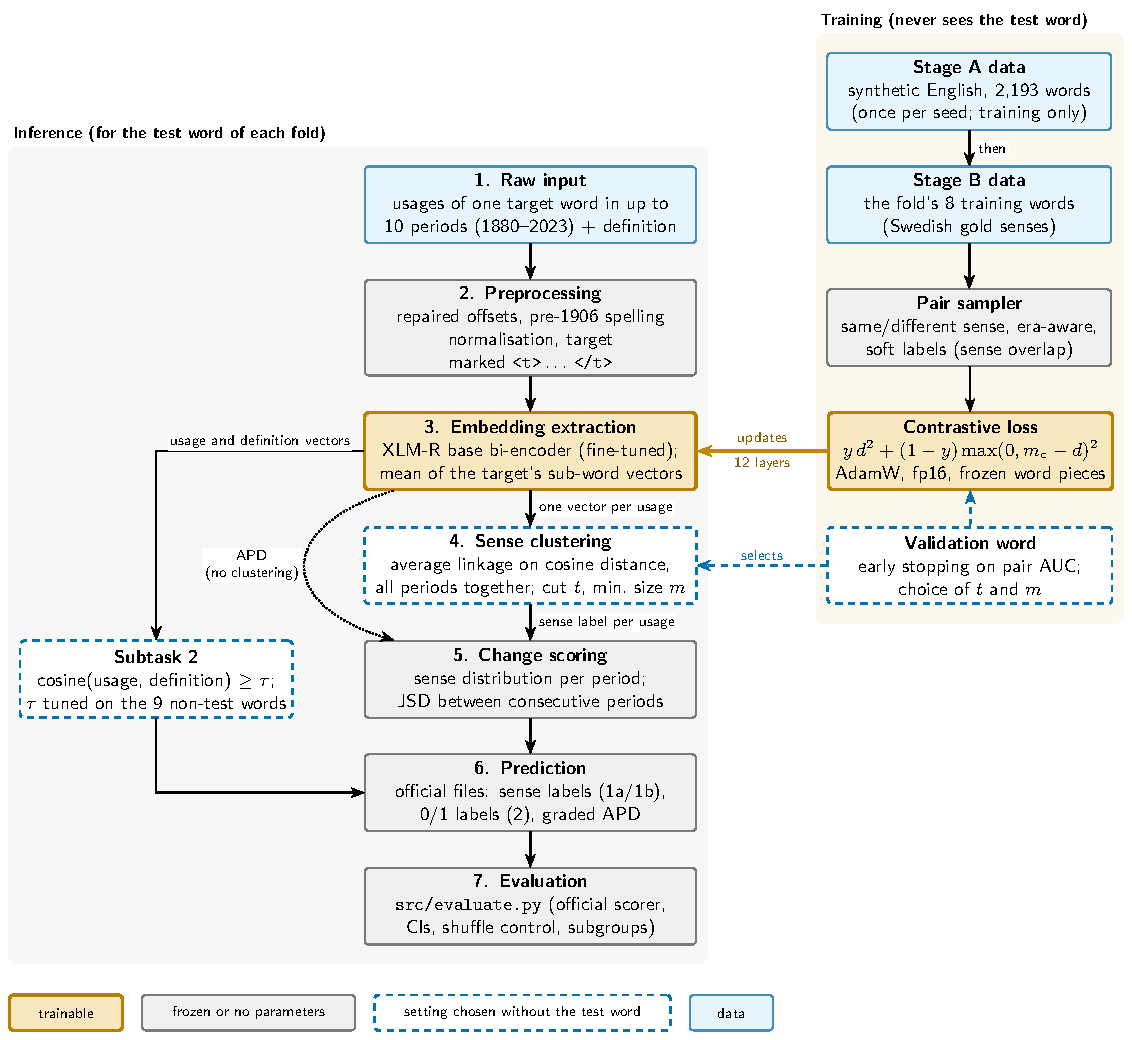
\includegraphics[width=\linewidth]{figures/architecture.pdf}
  \caption{Architecture of the proposed system. Orange: trainable (the XLM-R
  transformer layers, updated through the contrastive loss). Grey: frozen or
  parameter-free (preprocessing, word-piece embeddings, change scoring,
  prediction, evaluation). Dashed blue: settings chosen on the validation word
  (early stopping, clustering cut $t$ and minimum size $m$) or on the nine
  non-test words (Subtask~2 threshold $\tau$). The dotted arrow is APD, which
  scores change directly from the usage vectors without clustering.}
  \label{fig:architecture}
\end{figure}

\paragraph{Components.}
\begin{enumerate}
  \item \textbf{Raw input.} The official files \texttt{usages.jsonl},
        \texttt{definitions.jsonl} and the gold files, read by the shared loader
        (\texttt{data\_loader.load\_and\_prepare}).
  \item \textbf{Preprocessing} (no parameters). Offset repair, spelling
        normalisation and target marking (Section~\ref{sec:approach-preprocessing}).
        Every system uses the same settings.
  \item \textbf{Embedding extraction} (\emph{trainable}). XLM-R base. The 12
        transformer layers (about 86M parameters) are fine-tuned, and the
        192M-parameter word-piece embedding matrix is frozen. Output: one
        768-dimensional vector per usage and per definition.
  \item \textbf{Sense clustering} (no learned parameters; two settings chosen on
        the validation word). Average-linkage agglomerative clustering over all
        periods of a word, cut at $t$, with minimum cluster size $m$.
  \item \textbf{Change scoring} (no parameters). Sense distributions per period,
        JSD between consecutive periods (Eq.~\ref{eq:jsd}), and APD from the
        vectors (Eq.~\ref{eq:apd}).
  \item \textbf{Prediction} (no parameters). Writes the official Subtask~1 and
        Subtask~2 files and the local graded APD file.
  \item \textbf{Evaluation} (shared script, never modified by the model code).
        Official scores with 95\% bootstrap confidence intervals over words, the
        cluster-size shuffle control for 1b, and subgroup tables (Section~6).
\end{enumerate}

\paragraph{Training path.} Stage~A (synthetic English) and Stage~B (the fold's
eight Swedish training words) feed the pair sampler, which produces soft-labelled
same/different-sense pairs. The contrastive loss (Eq.~\ref{eq:loss}) updates the
encoder. The validation word controls early stopping and the clustering
settings. Stage~A runs once per seed and is cached. Stage~B restarts from the
Stage~A weights in every fold, so no fold's model has seen its test word.

\paragraph{Frozen comparison system.} The pretrained baseline (Section~4) uses
the same diagram with the orange components replaced: XLM-R base is frozen,
layer~8 is read instead of the last layer, and no target markers are used,
because their embeddings would be untrained. The rest of the pipeline is
unchanged, so the frozen-versus-fine-tuned ablation (Section~5) differs only in
the encoder.

\begin{table}[ht]
\centering
\small
\begin{tabularx}{\linewidth}{@{}lXl@{}}
\toprule
\textbf{Component} & \textbf{What is learned or chosen, and on what data} & \textbf{Status}\\
\midrule
Word-piece embeddings & Nothing (kept from pretraining) & frozen\\
Transformer layers 1--12 & Weights; synthetic pairs, then the fold's 8 training words & trainable\\
Checkpoint (epoch) & Best pair AUC on the validation word & selected\\
Clustering $t$, $m$ & Validation word (pair separation, BCubed F1) & selected\\
Subtask~2 threshold $\tau$ & 9 non-test words (official macro F1) & selected\\
JSD, APD & Nothing (fixed formulas) & no parameters\\
\bottomrule
\end{tabularx}
\caption{What each component learns or chooses, and from which words. The test word is not used by any row.}
\label{tab:architecture-status}
\end{table}
